\documentclass[11pt]{article}

\usepackage[a4paper,margin=25mm,headheight=14pt]{geometry}
\usepackage{fontspec}
\usepackage{unicode-math}
\setmainfont{Times New Roman}
\setsansfont{Arial}
\setmonofont{Menlo}
\setmathfont{STIX Two Math}
\usepackage{microtype}
\usepackage{amsmath,amsthm,mathtools}
\usepackage{booktabs,tabularx,longtable,array}
\usepackage{enumitem}
\usepackage{xcolor}
\usepackage{tikz}
\usetikzlibrary{arrows.meta,positioning,fit,calc}
\usepackage{fancyhdr}
\usepackage{hyperref}

\definecolor{navy}{HTML}{17365D}
\definecolor{blue}{HTML}{2F5597}
\definecolor{lightblue}{HTML}{EAF1F8}
\definecolor{deepred}{HTML}{8B1E2D}
\definecolor{graytext}{HTML}{4A4A4A}
\hypersetup{colorlinks=true,linkcolor=navy,citecolor=deepred,urlcolor=blue,pdfauthor={Satoru Watanabe},pdftitle={Subjectivity Intersection Mathematics: A Common Pointed-Braid Source for Quantum History and Lorentzian Geometry}}

\newtheorem{theorem}{Theorem}[section]
\newtheorem{proposition}[theorem]{Proposition}
\newtheorem{lemma}[theorem]{Lemma}
\newtheorem{corollary}[theorem]{Corollary}
\theoremstyle{definition}
\newtheorem{definition}[theorem]{Definition}
\newtheorem{assumption}[theorem]{Assumption}
\theoremstyle{remark}
\newtheorem{remark}[theorem]{Remark}

\newcommand{\cH}{\mathcal{H}}
\newcommand{\cA}{\mathcal{A}}
\newcommand{\cC}{\mathcal{C}}
\newcommand{\Tr}{\operatorname{Tr}}
\newcommand{\id}{\mathbf{1}}
\newcommand{\dd}{\mathrm{d}}
\newcommand{\ad}{\operatorname{ad}}
\newcommand{\Ric}{\operatorname{Ric}}
\newcommand{\Span}{\operatorname{span}}
\newcommand{\rank}{\operatorname{rank}}
\newcommand{\Ker}{\operatorname{ker}}
\newcommand{\im}{\operatorname{im}}
\newcommand{\Lie}{\mathcal{L}}
\newcommand{\RC}{\mathcal{R}_{C}}

\pagestyle{fancy}
\fancyhf{}
\fancyhead[L]{\small\color{graytext}Common pointed-braid source and Lorentzian geometry}
\fancyhead[R]{\small\color{graytext}Working preprint v0.1}
\fancyfoot[C]{\thepage}

\setlength{\parindent}{0pt}
\setlength{\parskip}{0.65em}
\setlist{nosep,leftmargin=1.5em}

\title{\vspace{-1.2cm}\textbf{Subjectivity Intersection Mathematics:}\\[0.18em]\textbf{A Common Pointed-Braid Source for Quantum History and Lorentzian Geometry}\\[0.35em]\Large A fixed-finite conditional composition with relational backreaction}
\author{Satoru Watanabe\\\small Subjectivity Intersection Emergence Lab (SIEL)}
\date{Working preprint v0.1 --- 11 September 2026}

\begin{document}
\maketitle

\begin{center}
\fcolorbox{navy}{lightblue}{\parbox{0.91\linewidth}{\small
\textbf{Status.} This is a working theoretical preprint. The main result is conditional, fixed-finite, local to one regular patch, and valid on a nonzero short-time interval. It is not peer reviewed and does not establish an empirically validated theory of quantum gravity, absolute semiclassical gravity, or an ontological theory of subjectivity.}}
\end{center}

\begin{abstract}
We construct a single typed mathematical system in which a quantum history and initial Lorentzian geometry are read from one finite pointed-braid source, rather than supplied as unrelated models and coupled afterwards. The source is a fixed bipartite state on $\cH_A\otimes\cH_B$, with $\dim\cH_A=\dim\cH_B=125$, together with its Hamiltonian, endpoint split, cup mark, insertions, and Yang--Baxter-coherent transport. The reduced source state determines both a free Hamiltonian history and, under explicit covariance-cone and clock-reflection assumptions, a four-dimensional Lorentzian initial metric. Its endpoint-invisible correlation component is the categorical kernel of the two partial traces and cannot be reduced to either endpoint on a matched-control family.

After this creation datum, geometry and the joint source-field state are evolved as distinct variables in one coupled local system. A common interaction preserves the original source energy ledger, produces a relative scalar stress, and combines with a relation-polarized constitutive stress to backreact on the metric. Under stated regularity, gauge, cone, reference, and soldering assumptions, standard symmetric-hyperbolic theory yields a unique common short-time solution. The full typed output descends through Yang--Baxter-equivalent presentations, so no representative crossing word is selected as absolute inside the declared groupoid.

For physical contact we define a diffeomorphism-covariant, $C$-polarized curvature response. Seven timelike probe frames provide 42 relative-acceleration scalars; an exact rational rank calculation reconstructs all 20 algebraic Riemann degrees of freedom, with an exhibited 20-channel inverse of infinity norm $13/4$. The ideal detector recovers the curvature response and its nonzero initial slope. We also prove a conditional detector-cylinder cutoff theorem and show that its application presently first-fails because no compatible varying-cutoff tower of the complete coupled system has been defined. An intrinsic finite-source principle is therefore isolated as an explicit, falsifiable working hypothesis rather than hidden as a convergence claim.
\end{abstract}

\noindent\textbf{Keywords:} braid group; Yang--Baxter coherence; quantum geometry; Lorentzian metric; backreaction; relational observable; symmetric-hyperbolic system; finite source.

\section{Problem and claim}

Many quantum--geometry constructions begin with a quantum model and a spacetime model that have independent state spaces, independent clocks, or independently normalized energies. A coupling term can then connect them, but the coupling alone does not show that they arise from one mathematical source. The question addressed here is narrower and stricter:

\begin{quote}
Can the quantum history, the initial Lorentzian geometry, the relational component that mediates their coupling, and the subsequent backreaction be placed on one source-derived object without duplicating the source or selecting one braid presentation as absolute?
\end{quote}

The answer is conditional but constructive. The central result is a local composition theorem for a fixed finite source. Its content is stronger than compatibility of two separately specified models: all source readouts come from one joint state, the source Hamiltonian is counted once, the initial metric is generated from the same reduced state that carries the quantum history, and the coupled state and metric then evolve in one local initial-value problem.

The result also has strict boundaries. Braid relations do not by themselves select four dimensions, the physical clock soldering, the reflection coefficient used to obtain Lorentz signature, the relative gravitational source law, or the absolute units. The construction therefore separates four layers:

\begin{enumerate}
\item exact finite algebra and exact rational certificates;
\item conditional mathematical composition under explicit bridge assumptions;
\item an unadopted finite-source physical model with an operational discriminator;
\item ontological interpretation, which is not proved here.
\end{enumerate}

Classical braid groups and Yang--Baxter consistency provide the mathematical background for the path equivalences used below \cite{artin1947,yang1967,lamberadford1997}. The direct source theorem is Watanabe's pointed-unitary-braid result: it proves canonical all-finite-orders endpoint overlaps, bilateral positive contractions, pointed-unitary covariance, and compatibility with the declared shuffled tensor law \cite{watanabe2026braid}. The present paper uses that theorem as its Braid foundation and does not strengthen its scope. Local covariance and the initial-value structure of general relativity supply comparison standards for the field-theoretic and geometric parts \cite{brunetti2003,choquet2008}. The construction is not presented as a replacement for those frameworks.

\section{The fixed pointed-braid source}

\subsection{One source state and its endpoint readouts}

Let
\begin{equation}
  \cH_{\mathrm{src}}=\cH_A\otimes\cH_B,
  \qquad \cH_A=\cH_B=\mathbb{C}^{125}.
\end{equation}
The actual finite source state used throughout the composition is
\begin{equation}\label{eq:gamma0}
  \Gamma_0=\frac{100\id+D\otimes D}{1{,}562{,}500},
  \qquad \Tr D=0,\qquad \Tr(D^2)=216.
\end{equation}
It is normalized and has maximally mixed endpoint marginals,
\begin{equation}
  \Gamma_A=\Tr_B\Gamma_0=\frac{\id_{125}}{125},
  \qquad
  \Gamma_B=\Tr_A\Gamma_0=\frac{\id_{125}}{125}.
\end{equation}

The full source package also contains the original Hamiltonian $H$, a fixed endpoint split, the cup mark $M_0$, insertion data, polar data, and selected graded generators. These objects are transported together. None is reconstructed from a scalar summary of the state.

The coupled system has one joint state $\Sigma(t)$ on
\begin{equation}
  \cH_{\mathrm{src}}\otimes\cH_F,
  \qquad \Sigma(0)=\Gamma_0\otimes\rho_F,
  \qquad \Tr\rho_F=1.
\end{equation}
The time-dependent source state is only the readout
\begin{equation}\label{eq:reduced}
  \Gamma(t)=\Tr_F\Sigma(t).
\end{equation}
Thus $\Gamma$ is not a second dynamical copy.

\subsection{The endpoint-invisible correlation carrier}

For any normalized bipartite state $\Gamma$, define
\begin{equation}\label{eq:corr}
  c_\Gamma=\Gamma-\Gamma_A\otimes\Gamma_B,
  \qquad
  \cC_{\mathrm{corr}}=\Ker\Tr_A\cap\Ker\Tr_B
\end{equation}
inside the real vector space of trace-zero Hermitian joint variations. For the actual state,
\begin{equation}
  c_0=\frac{D\otimes D}{1{,}562{,}500},
  \qquad
  \Tr(c_0^2)=\frac{216^2}{1{,}562{,}500^2}>0.
\end{equation}

Let $p=(\Tr_B,\Tr_A)$. The inclusion
$\iota:\cC_{\mathrm{corr}}\hookrightarrow\mathrm{Herm}_0(\cH_A\otimes\cH_B)$
is the categorical kernel of $p$ in the declared finite-dimensional real-linear category: every $T:Z\to\mathrm{Herm}_0$ satisfying $pT=0$ factors uniquely through $\iota$. Moreover, every normalized joint state has the unique decomposition in Eq.~\eqref{eq:corr}.

This universal property is elementary finite bipartite mathematics; it is not uniquely braid-specific. The source-specific content enters through the actual state, cup, operators, and their simultaneous transport. A matched control with unchanged endpoint marginals but a rotated right correlation factor changes a fixed cup response by the exact amount $62/48{,}828{,}125$. Therefore that joint response cannot factor through either endpoint marginal alone. This is an operational nonfactorization result, not an ontological identification of $c_\Gamma$.

\subsection{Typed braid descent}

Let $\mathsf{Cross}$ be the free typed crossing groupoid generated by the allowed elementary crossings and let $\mathsf{Braid}$ be its quotient by Yang--Baxter, remote-commutation, inverse, and unit relations. A typed output functor $F$ includes the labelled source history, the joint source-field evolution, the energy ledger, the relation mark, initial soldering, the field, and the local geometric problem.

\begin{proposition}[Typed descent criterion]\label{prop:descent}
$F$ factors uniquely through $\mathsf{Braid}$ if and only if it maps both sides of every generating relation to the same typed output.
\end{proposition}

\begin{proof}
This is the quotient universal property. Necessity follows because equivalent words have one image in the quotient. Sufficiency follows because equality on generating relations makes $F$ constant on the generated congruence, hence defines a unique functor on the quotient.
\end{proof}

The actual even typed source satisfies the required relations in the fixed-finite scope. A non-Yang--Baxter unitary control fails: for a retained label $p=|000\rangle\langle000|$, the two relation words produce orthogonal projector images and
\begin{equation}
  \Delta_p=\|\operatorname{Ad}_{W_L}(p)-\operatorname{Ad}_{W_R}(p)\|_{\mathrm{HS}}^2=2.
\end{equation}
The ordinary flip also satisfies Yang--Baxter, so descent proves a coherence role for braid structure but not uniqueness of the concrete raw representation.

\section{Initial Lorentzian geometry from the same source}

\subsection{A four-plane and ten independent metric directions}

The graded-greedy covariance-cone rule begins with the distinguished grade-one Hamiltonian generator and repeatedly adjoins the least higher grade whose unordered pair sums remain distinct and whose required source pivots are nonzero and untruncated. Stopping at four directions gives
\begin{equation}
  (1,2,4,8),qquad
  V=\Span_{\mathbb{R}}\{H,U_2,U_4,U_8\}.
\end{equation}
The ten unordered pair sums are
\begin{equation}
  2,3,5,9,4,6,10,8,12,16,
\end{equation}
all distinct. An exact triangular-minor certificate gives rank ten for the metric Jacobian. With source grade $m=3$ and declared finite bound $J=83$, every selected pivot is untruncated because $m+16\le J$.

Four directions are required here because the target is a symmetric $4\times4$ tensor with ten components. This stopping rule is an explicit construction choice; it is not a theorem that bare braid relations force four spacetime dimensions.

\subsection{Covariance cone and Lorentz signature}

For selected source generators $G_a$ and a clock operator $O_0$, define the centered covariance tensor
\begin{equation}
  K_{ab}=\Tr\Gamma\,\Delta Z_a\Delta Z_b,
  \qquad h_{ab}=\Re K(G_a,G_b),
\end{equation}
and clock response
\begin{equation}
  v_a=-2\Im K(G_a,O_0).
\end{equation}
At the actual base point, the exact response is
\begin{equation}
  v=(17/4,0,0,0).
\end{equation}
Normalize
\begin{equation}
  \theta=\frac{v}{\sqrt{v^{\mathsf T}h^{-1}v}}
\end{equation}
and impose the declared clock reflection
\begin{equation}\label{eq:lorentzmetric}
  g_0=h-2\,\theta\otimes\theta.
\end{equation}
Then $g_0$ has signature $(-,+,+,+)$, and
\begin{equation}
  K_{\mathrm{cov}}=\{x:\theta(x)\ge0,\ g_0(x,x)\le0\}
\end{equation}
is closed, convex, pointed, and full dimensional. Its $\theta=1$ section is a nondegenerate solid $h$-ellipsoid in $\Ker\theta$.

Equation~\eqref{eq:lorentzmetric} is a source-internal Lorentz construction. Equality with a separately measured natural light cone is not proved. The geometry map will be denoted $G$, so the typed initial creation identity is
\begin{equation}\label{eq:creation}
  g_0=G(\Gamma_0)=G(\Tr_F\Sigma_0).
\end{equation}

\section{One quantum--geometry evolution}

\subsection{Clock and energy soldering}

Three clock descriptions occur: the original $H$-evolution parameter $t$, the source covector $\theta$, and a material scalar $T$ in the local field system. Their physical identity is not a consequence of the braid relations. We impose the explicit noncircular soldering condition along one timelike anchor $\gamma$,
\begin{equation}\label{eq:clock}
  T(\gamma(t))=t,qquad u(T)=1,qquad \dd T\parallel\theta\quad\text{initially}.
\end{equation}

The source energy is counted once:
\begin{equation}\label{eq:energy}
  e(\Sigma)=\frac12\Tr\!\left[\Sigma(H\otimes\id_F)\right]
  =\frac12\Tr(\Gamma H).
\end{equation}
For vanishing coupling, the full source algebra follows the original free history
\begin{equation}
  \alpha_t^H(a)=e^{itH}a e^{-itH}.
\end{equation}
At nonzero coupling, the joint history is not identified with $\alpha_t^H$ on source words that do not commute with $H$.

\subsection{A common interaction and relative stress}

The retained local linear interaction is
\begin{equation}\label{eq:interaction}
  S_{\mathrm{int}}=-\lambda\int \chi(T)\,H\otimes\phi\;\dd T\wedge N,
\end{equation}
where $N$ is the local current three-form and $\chi$ is fixed in advance. Only the abelian charge algebra $C^*(H)$ enters spacelike local densities; the full noncommutative source remains on one timelike defect. The interaction commutes with $H\otimes\id_F$, preserving Eq.~\eqref{eq:energy} and the $H$-sector populations. On a fixed smooth background, the spectral sectors of $H$ give retarded affine scalar shifts and a controlled-Weyl joint propagator.

The geometric source is relative. For an advance-fixed reference state and the same metric and prescription, define
\begin{equation}
  \Delta T_\phi[g;\Sigma,\Sigma_{\mathrm{ref}}]
  =T_\phi[g,\Sigma]-T_\phi[g,\Sigma_{\mathrm{ref}}].
\end{equation}
Common state-independent geometric counterterms cancel in the difference. The proposed finite-model field equation is
\begin{equation}\label{eq:gravity}
  E_c[g]=G[g]+\Lambda g
  =\kappa\left(\Delta T_\phi+T_{\mathrm{mat}}+2\Pi\right).
\end{equation}
This is the \emph{Intersection-Relative Gravity} working law. It is a constitutive proposal, not a derived absolute semiclassical Einstein equation. Standard semiclassical gravity also couples quantum stress to classical geometry, but the well-definedness, renormalization, and backreaction problem is delicate \cite{hollandswald2001,pinamontisiemssen2021,meda2026}.

\subsection{Relation polarization and reciprocal backreaction}

The cup-marked relation selects an energy-tangent source direction $\Xi_C$. The geometry differential and spatial projection define
\begin{equation}\label{eq:dc}
  d_C=P_{\mathrm{sp}}DG\,\Xi_C.
\end{equation}
At the actual base point, one exact projected coordinate lies in the strictly negative interval
\begin{equation}
  -\frac{1127}{50{,}000{,}000{,}000}
  \le Dq[\Xi_C]\le
  -\frac{563}{25{,}000{,}000{,}000},
\end{equation}
so $d_C\ne0$. The relation enters as a zeroth-order target shift,
\begin{align}
  m_{\mathrm{sp}}^{\mathrm{RP}}
  &=P_{\mathrm{sp}}(w-DG\,X_H)-d_C,\\
  \frac{8K}{\rho}D_u^P\Pi+\Pi
  &=-K m_{\mathrm{sp}}^{\mathrm{RP}}.\label{eq:rp}
\end{align}
The source row retains the original intrinsic generator,
\begin{equation}
  D_u^B\Gamma=(I-P_H)X_H+R_E\Lie_u g,
\end{equation}
and the relation mark is transported by $D_uM=0$. On the regular patch, $d_C$ depends smoothly and algebraically on $(\Gamma,g,M)$. Consequently the feedback loop is
\begin{equation}\label{eq:loop}
  (M,\Gamma)\longrightarrow d_C\longrightarrow\Pi
  \longrightarrow g\longrightarrow\Gamma.
\end{equation}
The coefficient of $d_C$ in Eq.~\eqref{eq:rp} is a bold constitutive choice. It is not uniquely selected by the braid relations.

\subsection{Emergent-then-autonomous geometry}

The equality in Eq.~\eqref{eq:creation} is imposed only at the creation/soldering datum. Afterwards $g$ and $\Sigma$ are distinct state variables of the same coupled system. Requiring $g=G(\Tr_F\Sigma)$ at every time would both reduce geometry to an algebraic readout and conflict with the retained sector structure. The post-creation state space therefore realizes provenance without permanent algebraic identity.

The first-order variables are the generalized-harmonic metric block, the material clock/current and RP stress, the linear scalar field block, one finite joint-state block, and the transported relation mark. After the obsolete all-time matching row is removed, the principal symbol is a triangular direct sum of symmetric-hyperbolic and finite-dimensional blocks. Relative stress and exchange currents are lower-order locally Lipschitz functions on the stated weighted patch.

\section{The conditional local composition theorem}

We collect the construction into five conditions.

\begin{description}[leftmargin=3.2em,style=nextline]
\item[M1] The actual source state, $H,U_2,U_4,U_8$, $\theta$, $K_{\mathrm{cov}}$, and $g_0$ define the source-internal Lorentz carrier under the graded-greedy and reflection assumptions.
\item[M2$'$] The creation square $g_0=G(\Tr_F\Sigma_0)$ holds. Geometry and the joint state then coevolve without all-time algebraic identification.
\item[M3$^*$] The relation object is the correlation kernel $\cC_{\mathrm{corr}}$, its actual point $c_\Gamma$, and the existing cup mark $M_0$ required for relation transport.
\item[M4$'$] One timelike-defect source carries the same joint state, original $H/2$ ledger, local interaction, relative field stress, and relation-polarized constitutive stress.
\item[M5$'$] The combined system satisfies the regularity, constraint, cone, reference, and clock-soldering assumptions required for one common short-time solution.
\end{description}

\begin{theorem}[Pointed Correlation-Kernel Braid Quantum--Geometry Local Composition]\label{thm:main}
Assume M1--M5$'$ and the fixed-finite source identities above. For $s>5/2$ and compatible smooth initial data in one regular generalized-harmonic patch, there is a nonzero interval $[0,T_*]$ on which a unique local solution carries one joint state $\Sigma$, one reduced source readout $\Gamma$, the original Hamiltonian ledger counted once, the endpoint-invisible correlation carrier, the source-generated initial Lorentzian metric, the local quantum interaction, and relative geometric backreaction. If the complete typed data are transported simultaneously, Yang--Baxter-equivalent words define isomorphic typed histories and the same local solution problem.
\end{theorem}

\begin{proof}
The initial identity follows from Eq.~\eqref{eq:reduced} and Eq.~\eqref{eq:creation}. The correlation-kernel factorization and endpoint nonfactorization establish the M3$^*$ readout without adding a second state. Equation~\eqref{eq:interaction} preserves the single $H/2$ ledger and recovers the original $H$ history at zero coupling. Equations~\eqref{eq:gravity}--\eqref{eq:rp}, together with the material and exchange-current equations, form the retained triangular symmetric-hyperbolic plus finite-dimensional system. Its positive symmetrizer, local Lipschitz lower-order maps, compatible initial constraints, and strict cone margin give local existence, uniqueness, continuous dependence, and constraint propagation by standard quasilinear theory \cite{choquet2008}. Proposition~\ref{prop:descent} then transfers the full typed system to the braid quotient. No separate source state or second Hamiltonian is introduced.
\end{proof}

\begin{remark}[Meaning of ``same source'']
The theorem does not merely use the same parameter names in two models. The quantum and geometric sectors share the actual reduced state, clock soldering, energy ledger, relation mark, interaction history, and local solution. Removing any one of these identifications would weaken the result to compatibility or coupling of separate models.
\end{remark}

\section{A nonzero geometric response}

Compare two matched solutions of Eq.~\eqref{eq:gravity}: $\eta=1$ retains $d_C$ in Eq.~\eqref{eq:rp}, while $\eta=0$ removes only that term. Initial state, metric, first metric data, field, reference, material variables, $\Pi$, and gauge are identical. Then
\begin{equation}
  D_u^P(\Pi_1-\Pi_0)|_0=\frac{\rho}{8}d_C,
\end{equation}
and hence
\begin{equation}\label{eq:stressslope}
  D_u\Delta(2\Pi)|_0=\frac{\rho}{4}d_C\ne0.
\end{equation}
For smooth data, the two relative source histories therefore separate on every sufficiently short punctured interval.

Let $S=\Ker\theta$ carry the positive screen metric and transport $d_C$ along the material clock curve $\gamma(T)$. For any spatial tensor $X$, define
\begin{equation}
  P_C(X)=\frac{\langle d_C,X\rangle_S}{\langle d_C,d_C\rangle_S}.
\end{equation}
The relational curvature response is
\begin{equation}\label{eq:RC}
  \RC(T)=P_C\!\left(E_c[g_1]-E_c[g_0]\right)\big|_{\gamma(T)}.
\end{equation}
All indices are contracted and the branches are compared at equal material-clock value. Thus $\RC$ is invariant under simultaneous diffeomorphism and screen-frame change within the declared transport scope. From Eq.~\eqref{eq:stressslope},
\begin{equation}\label{eq:RCslope}
  D_T\RC(0)=\frac{\kappa\rho}{4}\ne0
\end{equation}
for $\kappa\ne0$ and $\rho>0$.

Equation~\eqref{eq:RCslope} is a model-internal discriminator. It does not show that the proposed relative source law is realized in nature; another covariant constitutive theory may reproduce the same local slope.

\section{Finite relational curvature readout}

\subsection{Seven probe frames}

At the equal-clock event, choose a transported orthonormal tetrad
\begin{equation}
  e_0=u,qquad e_1,e_2,e_3\in S.
\end{equation}
Use seven future unit-timelike velocities
\begin{equation}
  v_0=e_0,qquad
  v_i^{\pm}=\frac53e_0\pm\frac43e_i,quad i=1,2,3.
\end{equation}
For each velocity, choose an adapted orthonormal separation triple in $v^\perp$ and read the symmetric Jacobi bilinear form
\begin{equation}
  J_v(w,z)=R(w,v,z,v).
\end{equation}
Each frame yields six scalars, for 42 raw readings.

\begin{proposition}[Finite Riemann reconstruction]\label{prop:detector}
The exact rational linear map from the 20-dimensional space of algebraic four-dimensional Riemann tensors to the 42 Jacobi readings has rank 20. A selected 20-channel square subsystem has an inverse $L$ satisfying
\begin{equation}
  \|L\|_\infty=\frac{13}{4}
\end{equation}
in the declared tetrad-coordinate norm.
\end{proposition}

The remaining 22 readings are consistency checks. The reconstructed Riemann tensor gives $\Ric$, scalar curvature, and $E_c$. Contracting the branch difference with $d_C$ exactly recovers Eq.~\eqref{eq:RC} in the zero-size, zero-noise, zero-backreaction limit. For the exact response fixture used in the certificate,
\begin{equation}
  D_TD_C^{\mathrm{probe}}(0)=\frac{35}{132}=\frac{\kappa\rho}{4}.
\end{equation}

The probes carry only velocities, separations, small classical stresses, and metric readouts. They do not copy the noncommutative source algebra into spacelike regions.

\subsection{Finite error ledger}

If $\varepsilon$ is probe separation, $n_a$ bounds unnormalized acceleration noise, $\delta_T$ is clock resolution, and $m_{\mathrm{det}}$ measures probe stress, then on a regular patch the first symbolic bound is
\begin{align}\label{eq:error}
 |D_C^{\mathrm{meas}}-\RC^{J}|
 &\le C_{\mathrm{rec}}
 \left(\varepsilon\|\nabla\mathrm{Riem}\|+\frac{n_a}{\varepsilon}\right)\\
 &\quad+C_T\delta_T\|\nabla_uE_c\|+C_{\mathrm{br}}m_{\mathrm{det}}.
\end{align}
The reconstruction part is finite because of Proposition~\ref{prop:detector}; numerical values for the remaining patch and apparatus constants are not yet supplied. At fixed $n_a$, taking $\varepsilon\to0$ increases $n_a/\varepsilon$, so the ideal limit is not automatically an experimentally accessible limit.

\section{Cutoff relevance and the finite-source hypothesis}

\subsection{A conditional detector-cylinder theorem}

Suppose, beyond the fixed model already defined, that complete models indexed by $J$ are connected by typed embeddings. Let $\epsilon_J$ bound every adjacent defect relevant to the initial data, Hamiltonian, cup, clock, geometry map, $d_C$, and constitutive coefficients.

\begin{theorem}[Detector-cylinder summable stability]\label{thm:cutoff}
Assume $\sum_{J\ge J_0}\epsilon_J<\infty$. Assume further that all models share a nonzero interval $I=[0,T]$, a uniform cone margin, symmetrizer bounds, Sobolev bounds, local Lipschitz constant $L$, a positive uniform lower bound for $\|d_C^J\|$, and a uniformly Lipschitz 42-reading map with constant $C_D$. Then
\begin{equation}\label{eq:cauchy}
 \sup_{t\in I}\|Y_K(t)-Y_J(t)\|
 \le C_D(1+T)e^{LT}\sum_{n=J}^{K-1}\epsilon_n.
\end{equation}
Consequently $Y_J$ and $\RC^J$ are uniformly Cauchy on $I$.
\end{theorem}

\begin{proof}
Let $E_{JK}(t)$ be the embedded difference norm for the two local solutions. The standard difference-energy estimate has the form
\begin{equation}
 E_{JK}(t)\le a_{JK}+\int_0^t\left(LE_{JK}(s)+b_{JK}\right)\dd s,
\end{equation}
where the telescoped adjacent defects give
$a_{JK},b_{JK}\le\sum_{n=J}^{K-1}\epsilon_n$.
Gronwall's inequality yields
\begin{equation}
 \sup_I E_{JK}\le(1+T)e^{LT}\sum_{n=J}^{K-1}\epsilon_n.
\end{equation}
Composition with the uniformly Lipschitz detector and normalized $d_C$ contraction gives Eq.~\eqref{eq:cauchy}. Summability makes its right side vanish as $J,K\to\infty$.
\end{proof}

The theorem avoids convergence of every source component. It is nevertheless not presently applicable to the actual model: no authoritative construction defines the complete compatible family of joint state, source algebra, $H$, cup, clock, geometry map, dynamic $d_C$, constitutive coefficients, and local solution for varying $J$. The initial inequality $m+16\le J$ controls only the ten initial metric pivots. Because $d_C=d_C(\Gamma,g,M)$ evolves inside the feedback loop, initial nontruncation does not imply equality of finite-time detector histories.

\subsection{Intrinsic Finite Braid Source Principle}

The shortest live route therefore isolates the following hypothesis.

\begin{assumption}[Intrinsic Finite Braid Source Principle, IFBSP]\label{ass:ifbsp}
The declared actual source with $J_*=83$ is the internal Braid source of the model, rather than a regulator approximation to an otherwise specified $J=\infty$ source. The Lorentzian spacetime and scalar field remain continuous; only the internal Braid-source sector is intrinsically finite.
\end{assumption}

IFBSP is noncircular: it fixes the model class before calibration or held-out validation and assumes neither Eq.~\eqref{eq:RCslope} as an empirical fact nor agreement with data. Under IFBSP, the theoretical observable is $\RC^{83}$ and Eq.~\eqref{eq:error} contains no undefined $\RC^\infty$ residual. This is a finite-theory choice, not a proof of cutoff convergence.

The assumption is falsified as a working route if $J_*$ is retuned after outcomes, if the source definition is shown to require a separately specified infinite object, if a required source identity fails at $J_*$, if the intended claim requires $J\to\infty$ universality, or if independent prospective tests reject the frozen finite-source predictions.

\section{Physical scales and a no-retuning protocol}

The internal equations are dimensionless and retain two continuous scale freedoms. Let $\tau_*$ be the physical duration of one internal clock unit and $\sigma_*$ the physical stress associated with one internal stress unit. Then
\begin{align}
 t_{\mathrm{phys}}&=\tau_*T,&
 x_{\mathrm{phys}}&=c\tau_*x,\\
 H_{\mathrm{phys}}&=\frac{\hbar}{\tau_*}H,&
 T_{\mathrm{phys}}&=\sigma_*T,\\
 (E_c)_{\mathrm{phys}}&=\frac{E_c}{(c\tau_*)^2},&
 \kappa_{\mathrm{phys}}&=\frac{\kappa}{\sigma_*(c\tau_*)^2}.
\end{align}
Rescaling $\tau_*$ and $\sigma_*$ leaves every dimensionless braid word, state, cone, and $\RC(T)$ unchanged. Bare internal mathematics therefore cannot determine absolute seconds, metres, or gravitational strength.

Choose in advance one nonzero dimensionless gap $\Delta h_{\mathrm{cal}}$ and an independently measured angular frequency $\omega_{\mathrm{cal}}$, and one independent physical gravitational-coupling anchor $\kappa_{\mathrm{cal}}$. Then
\begin{equation}
 \tau_*=\\frac{\Delta h_{\mathrm{cal}}}{\omega_{\mathrm{cal}}},
 \qquad
 \sigma_*=\frac{\kappa}{\kappa_{\mathrm{cal}}(c\tau_*)^2}.
\end{equation}
These two relations locally fix the two logarithmic scale freedoms. They must not use the held-out $C$-polarized response.

Before any outcome access, a prospective packet must freeze the source revision, $J_*$, state, $H$ gap, dimensionless couplings, density convention, clock and screen soldering, reference prescription, detector map, apparatus error domain, and success rule. Post-outcome changes define a new exploratory model.

\section{What braid coherence contributes}

The mathematical role of braid structure in this paper is neither ``noncommutativity alone'' nor the claim that every quantum--gravity model must be braided. Building on the pointed-unitary-braid theorem \cite{watanabe2026braid}, its concrete contribution here is commutation of construction with viewpoint transport:
\begin{equation}
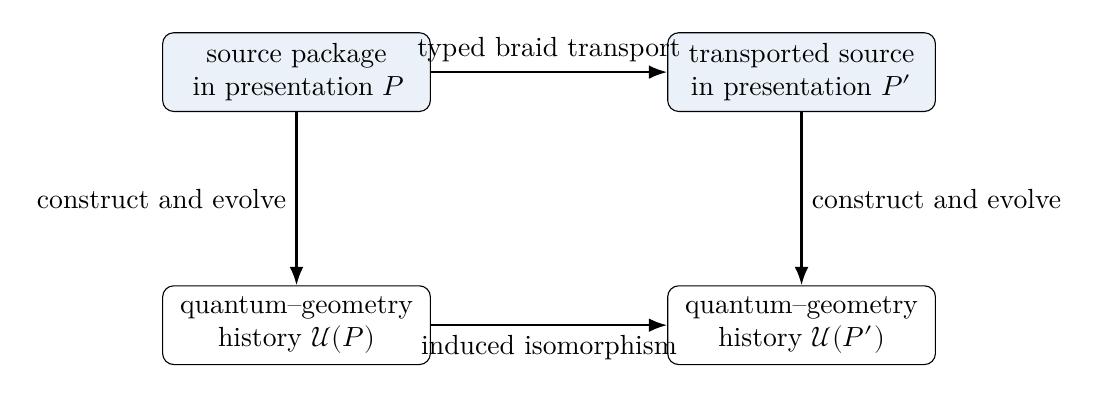
\begin{tikzpicture}[baseline=(current bounding box.center),node distance=22mm and 30mm,>=Latex]
\node[draw,rounded corners,fill=lightblue,align=center,minimum width=34mm,minimum height=10mm] (s) {source package\\in presentation $P$};
\node[draw,rounded corners,fill=lightblue,align=center,right=of s,minimum width=34mm,minimum height=10mm] (sp) {transported source\\in presentation $P'$};
\node[draw,rounded corners,fill=white,align=center,below=of s,minimum width=34mm,minimum height=10mm] (u) {quantum--geometry\\history $\mathcal U(P)$};
\node[draw,rounded corners,fill=white,align=center,below=of sp,minimum width=34mm,minimum height=10mm] (up) {quantum--geometry\\history $\mathcal U(P')$};
\draw[->,thick] (s)--node[above]{typed braid transport}(sp);
\draw[->,thick] (s)--node[left]{construct and evolve}(u);
\draw[->,thick] (sp)--node[right]{construct and evolve}(up);
\draw[->,thick] (u)--node[below]{induced isomorphism}(up);
\end{tikzpicture}
\end{equation}
Applying a viewpoint change before constructing the geometry and dynamics gives the same typed result as constructing first and transporting the entire result. State, $H$, cup, clock, $d_C$, soldering, metric, and equations must all move together. Moving only one part defines a different experiment.

This is the precise sense in which no crossing word or matrix presentation is absolute inside the allowed groupoid. A labelled non-Yang--Baxter control fails the full typed equalizer, demonstrating that the relation is not vacuous. Yet the metric-only projection can miss that failure, and the ordinary flip can satisfy the same coherence relation. Braid coherence is therefore sufficient for the declared descent and detected by a faithful full output, while concrete physical uniqueness remains open.

The broader Subjectivity-Intersection programme motivates interpreting an irreducible reciprocal relation as a candidate ``third standpoint'' \cite{watanabe2026ontology,watanabe2026sim}. No such ontology is used in the proof. In particular, mathematical standpoint data are not phenomenal consciousness, and neither light nor a quantum system is called conscious here.

\section{Countermodels, negative results, and claim boundaries}

The route was narrowed by explicit failures that remain part of the result.

\begin{longtable}{>{\raggedright\arraybackslash}p{0.17\linewidth}>{\raggedright\arraybackslash}p{0.34\linewidth}>{\raggedright\arraybackslash}p{0.39\linewidth}}
\toprule
Boundary & Failure or limitation & Consequence retained in the present model\\
\midrule
\endfirsthead
\toprule
Boundary & Failure or limitation & Consequence retained in the present model\\
\midrule
\endhead
Local source cloning & Two spacelike regions cannot each implement the full noncommutative source on one code while maintaining microcausality. & The full source lives on one timelike defect; spacelike probes read only metric curvature.\\
Nonlinear local packet & The examined spatially extended bounded nonlinear Weyl packet has a strict-locality counterexample. & The retained interaction is the evaluated local linear Same-$H$ model.\\
All-time metric readout & Fixed $H$-sector populations conflict with demanding ten independent moving-state metric controls at every time. & Geometry is source-generated initially and autonomous thereafter, with reciprocal coupling.\\
Absolute stress & The examined absolute reference-stress closure does not supply the required second-order local system. & The present source law uses a matched same-reference stress difference and states this constitutive choice openly.\\
Metric-only braid test & A non-Yang--Baxter source defect can vanish after projection to a matched local field stress. & Braid descent is claimed for the full labelled typed object, not as a unique metric-only signature.\\
Infinite cutoff & The complete varying-$J$ coupled tower is not defined. & The convergence theorem is conditional; IFBSP supplies a separate finite-source route.\\
Empirical status & No frozen external calibration or independent detector dataset has been evaluated. & The result remains theoretical and conditionally formulated.\\
\bottomrule
\end{longtable}

The paper therefore does not establish any of the following: a unique derivation of four dimensions from braid relations; equality with the observed light cone; an absolute renormalized stress law; a continuum or large-$N$ limit; numerical apparatus feasibility; empirical quantum gravity; an ontological identity between the correlation kernel and physical space; SIC/O3; subjectivity; or consciousness.

\section{Reproducibility and provenance}

The exact finite certificates were produced from versioned computational records. The main checks used by this manuscript are listed in Table~\ref{tab:certificates}. Hashes refer to the local research snapshot from which working preprint v0.1 was generated. Public replication requires a separately released verification bundle; this PDF alone is not a complete independent replication package.

\begin{table}[ht]
\centering
\small
\caption{Core internal certificates summarized in working preprint v0.1.}
\label{tab:certificates}
\begin{tabularx}{\linewidth}{@{}lXl@{}}
\toprule
Record & Certified content & Status\\
\midrule
UB300 & Actual state identity and nonzero same-energy relation response & exact finite\\
UB303 & Original-$H$ compatible relation-polarized repair and feedback typing & exact/conditional\\
UB317/328 & Full typed Yang--Baxter descent and labelled non-YB control & exact/conditional\\
UB333 & Four source directions, Lorentz carrier, ten-pivot rank certificate & exact/conditional\\
UB336 & Correlation-kernel universal property and endpoint nonfactorization & exact finite\\
UB337 & Same-object M1--M5$'$ composition audit & conditional theorem\\
UB338/339 & Nonzero stress-to-curvature response and relational scalar & exact/conditional\\
UB340 & Two-scale underidentification and no-retuning map & exact algebraic\\
UB341 & 42-to-20 Riemann reconstruction, inverse norm $13/4$ & exact finite\\
UB342 & Conditional cutoff theorem and actual tower-definition first-fail & conditional theorem/audit\\
\bottomrule
\end{tabularx}
\end{table}

Standard ingredients are not claimed as original. They include braid groups, the Yang--Baxter relation, partial traces, geodesic deviation, generalized-harmonic reduction, Gronwall estimates, and symmetric-hyperbolic local theory. The project-specific synthesis, source realization, typed composition, and exact certificates were developed through an iterative human-directed research process assisted by OpenAI Codex. The author is responsible for checking the mathematics, claims, citations, and public release. This v0.1 record preserves derivation assistance rather than treating the software as an intellectual source.

\section{Discussion}

The strongest conclusion is architectural. The construction demonstrates that a fixed finite quantum source can do more than source a metric through an externally chosen expectation value. The same reduced state participates in the free quantum history, creates the initial covariance cone and Lorentz metric, supplies the irreducible correlation readout, fixes a relation polarization through the cup mark, and remains inside the joint state that exchanges influence with the geometry. The backreaction loop is therefore internal to one typed object.

This common provenance matters because formal coupling is cheap: two independently defined theories can almost always be joined by adding an interaction term. The present theorem imposes stronger bookkeeping. There is one source state, one Hamiltonian ledger, one clock soldering, one initial creation map, one relation package, and one local solution. Those identities are precisely what would fail if the quantum and geometric sectors were unrelated copies.

The viewpoint claim is also scoped. Yang--Baxter equivalence ensures that the complete construction does not depend on which representative crossing word is used. This supplies a concrete consistency mechanism for avoiding an absolute presentation. It does not show that there are no other coherence mechanisms, nor that mathematical presentations are themselves subjects.

The decisive next scientific step is empirical rather than another dense internal enumeration. IFBSP freezes the finite source as the theory object. A prospective study must then use independent scale anchors and test a held-out $C$-polarized response or cross-context ratio with predeclared apparatus tolerances. A failure must remain a failure; changing $J_*$, the reference state, coupling, or detector channel afterwards creates a new model.

\section{Conclusion}

We have given a conditional, fixed-finite local theorem in which quantum history and initial Lorentzian geometry arise from one pointed-braid source and subsequently evolve with reciprocal backreaction in one system. The endpoint-invisible correlation carrier is endogenous to the actual source state, the original source energy is counted once, and the full typed construction descends through Yang--Baxter-equivalent presentations. A finite relational detector reconstructs local curvature and recovers a nonzero model-internal response.

The result is a mathematical unification architecture, not an empirically completed theory of quantum gravity. Its strongest unresolved assumptions are the operational identification of the source cone and clock, the constitutive relative-gravity law, the intrinsic finite-source hypothesis, physical calibration, and independent validation. Making those assumptions explicit turns them into targets for falsification instead of concealing them inside the word ``unification.''

\section*{Data and code availability}

This working preprint reports exact finite certificates and versioned internal audit records. A public verification bundle has not yet been deposited with v0.1. The absence of that bundle limits independent reproducibility and will be addressed in a later version if the source materials are approved for release.

\section*{Competing interests}

The author declares no competing interests.

\section*{Funding}

No external funding is declared for this working preprint.

\section*{AI assistance disclosure}

OpenAI Codex was used under the author's direction for mathematical ideation, derivation assistance, exact-check scripting, audit organization, and drafting. The author retains responsibility for verification, interpretation, citations, and the decision to release this version.

\begin{thebibliography}{99}

\bibitem{artin1947}
E. Artin, ``Theory of braids,'' \emph{Annals of Mathematics} \textbf{48}(1), 101--126 (1947). \href{https://doi.org/10.2307/1969218}{doi:10.2307/1969218}.

\bibitem{yang1967}
C. N. Yang, ``Some exact results for the many-body problem in one dimension with repulsive delta-function interaction,'' \emph{Physical Review Letters} \textbf{19}, 1312--1314 (1967). \href{https://doi.org/10.1103/PhysRevLett.19.1312}{doi:10.1103/PhysRevLett.19.1312}.

\bibitem{lamberadford1997}
L. A. Lambe and D. E. Radford, \emph{Introduction to the Quantum Yang--Baxter Equation and Quantum Groups: An Algebraic Approach}. Springer (1997). \href{https://doi.org/10.1007/978-1-4615-4109-7}{doi:10.1007/978-1-4615-4109-7}.

\bibitem{brunetti2003}
R. Brunetti, K. Fredenhagen, and R. Verch, ``The generally covariant locality principle---a new paradigm for local quantum field theory,'' \emph{Communications in Mathematical Physics} \textbf{237}, 31--68 (2003). \href{https://doi.org/10.1007/s00220-003-0815-7}{doi:10.1007/s00220-003-0815-7}.

\bibitem{hollandswald2001}
S. Hollands and R. M. Wald, ``Local Wick polynomials and time ordered products of quantum fields in curved spacetime,'' \emph{Communications in Mathematical Physics} \textbf{223}, 289--326 (2001). \href{https://doi.org/10.1007/s002200100540}{doi:10.1007/s002200100540}.

\bibitem{choquet2008}
Y. Choquet-Bruhat, \emph{General Relativity and the Einstein Equations}. Oxford University Press (2008). \href{https://doi.org/10.1093/acprof:oso/9780199230723.001.0001}{doi:10.1093/acprof:oso/9780199230723.001.0001}.

\bibitem{pinamontisiemssen2021}
N. Pinamonti and D. Siemssen, ``Existence and uniqueness of solutions of the semiclassical Einstein equation in cosmological models,'' \emph{Annales Henri Poincar\'e} \textbf{23}, 297--329 (2022). \href{https://doi.org/10.1007/s00023-021-01067-8}{doi:10.1007/s00023-021-01067-8}.

\bibitem{meda2026}
P. Meda, ``The semiclassical Einstein equations in cosmological spacetimes,'' \emph{International Journal of Theoretical Physics} \textbf{65}, 137 (2026). \href{https://doi.org/10.1007/s10773-026-06339-9}{doi:10.1007/s10773-026-06339-9}.

\bibitem{watanabe2026braid}
S. Watanabe, \emph{Subjectivity-Intersection Mathematics: All-Orders Intersection Consistency and Compositional Objectivity from Pointed Unitary Braids}, version 1.0, Zenodo (2026). \href{https://doi.org/10.5281/zenodo.22166167}{doi:10.5281/zenodo.22166167}.

\bibitem{watanabe2026ontology}
S. Watanabe, \emph{Subjectivity Intersection Ontology: A Comparative Ontological Framework for Third Subjectivity}, version 1.0.0, Zenodo (2026). \href{https://doi.org/10.5281/zenodo.21641878}{doi:10.5281/zenodo.21641878}.

\bibitem{watanabe2026sim}
S. Watanabe, \emph{Subjectivity-Intersection Mathematics Public Working Preprint v4.2 Draft}, Zenodo (2026). \href{https://doi.org/10.5281/zenodo.21909933}{doi:10.5281/zenodo.21909933}.

\end{thebibliography}

\end{document}
